\documentclass[12pt]{article}
%\documentclass[paper=a4]{scrartcl}
\usepackage{ucs}     % unicode 
\usepackage[utf8x]{inputenc}  % utf-8
\usepackage[ngerman]{babel}  % new german spelling 
\usepackage{graphicx}   % use graphics 
\usepackage{fancyhdr}   % header and footer
%\usepackage{scrpage2} 
\usepackage{setspace}
\usepackage{url}
\usepackage{tikz}
\usepackage{tikz-qtree}
\usepackage[printonlyused]{acronym}
\usepackage{a4wide} %depricated, use: geometry 
%\usepackage{cite}
\usepackage{natbib}	% bibstyle 
\usepackage[section]{placeins}	% \FloatBarrier
\usepackage[T1]{fontenc} %enable hyphenation for words including umlaute
\usepackage[pdfborder={0 0 0}]{hyperref} %links, aber ohne Rahmen
\usepackage{nameref} %Verweise auf sections
\usepackage{amsmath}
\usepackage{booktabs}

% Settings
\hyphenation{TIGER} % do not hyphenize
\bibpunct{[}{]}{,}{a}{}{;}


\setcounter{tocdepth}{2}
\begin{document}

\thispagestyle{empty} 

\begin{center}
	\topskip0pt
	\vspace*{\fill}
	
	\Huge{\textbf{Seminararbeit}}\\
	\vspace{1.5cm}
	
	\Large{\textbf{Automatische Bestimmung semantischer Rollen im deutschen
	Korpus SALSA 2.0}}\\
	\vspace{1cm}
		
	
\includegraphics[scale=0.3]{images/logo_hu.png}
	\vspace{1cm}

	\begin{Large}
		Institut für Informatik \& Institut für Linguistik\\
		Humboldt-Universität zu Berlin\\
		\vspace{1.5cm}
		Robert Bärhold \& Arne Binder \\
		31. März 2014 \\ %TODO
		\vspace{1cm}
		
		\begin{table}[h]
			\Large
			\centering
			\begin{tabular}{l l}
				Seminar: & Computergestützte Analyse von Sprache\\
				Seminarleiter: & Prof. Dr. Ulf Leser\\
				 		    & Prof. Dr. Anke Lüdeling \\
				Semester: & Wintersemester 2013/14 				 	
			\end{tabular}
		\end{table}	
	\end{Large}
	\vspace*{\fill}
\end{center}


\pagenumbering{roman}
\pagestyle{fancy} %eigener Seitenstil
\fancyhf{} %alle Kopf- und Fußzeilenfelder bereinigen
\renewcommand{\headrulewidth}{0pt} %obere Trennlinie
\renewcommand{\footrulewidth}{0pt} %untere Trennlinie 
\fancyfoot[C]{\thepage} %Seitennummer

 \newpage
 \tableofcontents
 \vspace{1cm}
 \listoffigures
 \vspace{1cm}
 \listoftables

\newpage
\pagenumbering{arabic}

\section{Einleitung}
- warum SRL? Motivation
- was gibt es schon? related work
[Shalmaneser, gildea \& jurafski, SEMAFOR, LTH, ...]
\subsection{Semantische Rollen}

Prädikate zeichnen sich dadurch aus, dass sie die Komplementationsstruktur einer
übergeordneten syntaktischen Einheit (nämlich des Satzes) bestimmen. Zum
Beispiel verlangt ein ditransitives Verb wie \glqq{}geben\grqq{} drei weitere Satzkonstituenten mit konkreten syntaktischen Eigenschaften:

\begin{center}
	\begin{tikzpicture}
		\Tree [.geben
				[.Subjekt Paul ]
				[.{} gibt ]
				[.Akk-Objekt {die Jacke} ]
				[.Dativ-Objekt {seiner Freundin} ]
			]
			
		%\Tree [.geben
		%		[.\textbf{Subjekt} Paul ]
		%		[.{} gibt ]
		%		[.\textbf{Akk-Objekt} {die Jacke} ]
		%		[.\textbf{Dativ-Objekt} {seiner Freundin} ]
		%	]
	\end{tikzpicture}
\end{center}

Aber das Bedingtheitsverhältnis zwischen dem Verb und seinen Komplementen 
endet nicht in der Syntax. Diese sind durch das Prädikat auch hinsichtlich ihrer 
\textit{semantischen} Integrierung in den Satz determiniert. Dem Komplement \glqq{}Paul\grqq{}
wird einmal die syntaktische Funktion des Subjekts zugewiesen, es wird aber auch
durch die konkrete Semantik der Handlung \glqq{}geben\grqq{} als 
\glqq{}Geber\grqq{} charakterisiert. Man spricht von den Argumenten
eines Verbs und sagt, dass sie \textit{semantische Rollen} realisieren. So realisiert \glqq{}Paul\grqq{} im obigen Beispiel die semantische Rolle \glqq{}Geber\grqq{}.

\subsection{Frame Semantik}

Die traditionelle Semantik [TODO: evtl. welche traditionelle Sem.? Referenz?] war versucht, eine möglichst abstrakte und
allgemeine, intersprachliche Formulierung von semantischen Rollen zu
finden - bei der man z. B. nicht von \glqq{}Geber\grqq{} sondern allgemein
von \glqq{}Agens\grqq{} sprechen würde. Demgegenüber steht die von C.J. Fillmore
ab den 70er Jahren entwickelte Theorie der Frame-Semantik (FS)
[\cite{fillmore1985}]. Das Fundament der Theorie ist mit dem traditionellen
Ansatz in höchstem Maße inkompatibel, für unser Vorhaben reicht es aber, die
partikuläre Auffassung von semantischen Rollen zu erwähnen, die der
Frame-semantische Ansatz mit sich bringt.

Rollen bzw. Frame-Elemente (FE) in Termini der FS werden nicht in Bezug auf die
Argumentstruktur von Verben formuliert, sondern hinsichtlich der globalen
Situation (oder des \textit{Frames}), die durch das Prädikat evoziert wird. Aufgrund
des situationellen Charakters der Frames sind nicht nur Verben sondern auch
Nomina (\textit{Mord}, \textit{Auge}\footnote{beispielsweise als Indikator für ein Ereignis der Wahrnehmung: \glqq{}Vor seinen Augen zerrissen sie die Bücher.\grqq{}}, \textit{Frau} von jemandem) oder Adjektive (\textit{stolz} auf etwas sein) potentielle
Frame-einführende Elemente, und in diesem Sinne auch Prädikate. Nachfolgend ist der Frame \glqq{}Kritik1-salsa\grqq{} dargestellt, so wie er im framesemantisch-annotierten SALSA 2.0 Korpus [\cite{rehbein_adding_2012}] definiert ist:

\begin{quote}
\textbf{Definition:}
A Reviewer offers his or her assessment of a work of art or performance (e.g. a play, a novel, a piece of music composition etc). The Reviewer typically bases his judgment on their own expertise and uses some set of criteria for evaluating works as to their relative merit.

\textbf{Example Sentences:}
\begin{enumerate}
\item Ich hab absichtlich auch noch keine anderen \textbf{Kritiken} gelesen und möglicherweise hab ich ein paar Dinge in dem Film übersehen.
\item Ich bin auf das Buch durch die \lbrack lobende\rbrack \textsuperscript{Valence} \textbf{Kritik} \lbrack in der FAZ\rbrack \textsuperscript{Medium} aufmerksam geworden.
\item \lbrack Olaf Storbecks Jahrhundertkrise\rbrack\textsuperscript{Evaluee}\lbrack erntet\rbrack\textsuperscript{Support} erste\lbrack gute\rbrack \textsuperscript{Valence} \textbf{Kritiken}.
\item Star Dreck - \lbrack Negative\rbrack \textsuperscript{Valence} \textbf{Kritiken} \lbrack von Fans\rbrack \textsuperscript{Reviewer}  \lbrack zum neuen Star Trek\rbrack \textsuperscript{Evaluee}
\end{enumerate}


\textbf{FEs}


\textbf{FE1(Reviewer)}: The person assessing the Evaluee for its merit.

\textbf{FE2(Evaluee)}: The cultural artifact that is evaluated.

\textbf{FE3(Medium)}: The venue or publication in which the review is distributed.

\textbf{FE4(Valence)}: The positive or negative nature of the evaluation, if specified. 
\end{quote}

\subsection{Semantic Role Labeling}\label{subsec:introduction_SRL}

Mit Semantic Role Labeling (SRL) ist die automatisierte Erkennung und
Annotierung von semantischen Rollen innerhalb eines Satzes gemeint. Die primäre
Aufgabe von SRL ist die genaue Identifizierung der semantischen Beziehung
zwischen einem Prädikat und seinen assoziierten Elementen und Eigenschaften
(siehe \cite{SRL2008} für eine allgemeine Darstellung). In Bezug auf eine FS lässt
sich folgendes feststellen. Da FE Frame-spezifisch sind, stellen sie eine
Zwischenstufe in der semantischen Abstraktion zwischen der rein lexikalischen
Bedeutung und den traditionellen Verbenübergreifenden [@Enrique: was meinst hier mit Verb..übergr.?] semantischen Rollen dar.
Die dadurch erreichte \glqq{}mildere\grqq{} Stufe der Abstraktion über die
Rollen der verschiedenen Verben, Nomina und Adjektive eignet sich besonders gut
für die Lösung unterschiedlicher Aufgabenstellungen in Bereichen des
Sprachverstehens [TODO: Leser konnte hiermit nichts anfangen :-( kann man das irgendwie erläutern/konkretisieren?] wie der Informationsextraktion oder Dialogsystemen [TODO: Verweis/Erklärung]. [\cite{gildea}]

[TODO kürzen und einbauen(an richtiger Stelle): The relationship between such surface manifestations and
semantic roles is the subject of linking theory—see \cite{levinrappaport}
for a synthesis of work in this area. In general, linking theory argues that the syntactic
realization of arguments of a predicate is predictable from semantics—exactly how this
relationship works is the subject of much debate. Regardless of the underlying mechanisms
used to generate syntax from semantics, the relationship between the two suggests
that it may be possible to learn to recognize semantic relationships from syntactic
cues, given examples with both types of information.]

Die Aufgabenstellung eines FS-orientierten SRL-Systems lässt sich im Allgemeinen
wie folgt untergliedern:
\begin{enumerate}
\item Zunächst wird der Frame, der durch den Satz oder die Phrase realisiert wird, bestimmt.
\item Es folgt die Bestimmung der Frame-Elemente bezüglich des Frames. 
\item Schließlich erfolgt die Klassifizierung der einzelnen Frame-Elemente.
\end{enumerate}


\section{Problemstellung}
Im Zuge dieser Arbeit soll die Frage geklärt werden, ob sich der Ansatz von \cite{gildea} auf einer Baumbank, das heißt einem Phrasen-annotierten Textkorpus, der deutschen Sprache adaptieren lässt. Dieser Ansatz besagt, dass mithilfe lexikalischer und syntaktischer Informationen verlässliche Annahmen über die Realisierung von semantischen Rollen durch Konstituenten eines Satzes getroffen werden können. Die Annahme lässt sich dazu nutzen, ein automatisiertes, statistisches Lernverfahren basierend auf einem zusätzlich mit Rollen annotierten Korpus zu entwickeln, welches die automatische Bestimmung der in einem deutschen Satz realisierten semantischen Rollen mit akzeptabler Genauigkeit ermöglicht.

\subsection{Korpus: Salsa 2.0}
Grundlage dieser Arbeit bildet das SALSA Korpus in der Version 2.0. Das SALSA Korpus ist ein für akademische Zwecke frei zugängliches, framesemantisch annotiertes Korpus der deutschen Sprache. Es basiert auf TIGER\citep{brants_tiger_2002, tiger}, einer Baumbank aus deutschen Zeitungsartikeln, welche semi-automatisch mit POS-Tags, Lemma-Informationen und syntaktischen Strukturen annotiert wurde.\footnote{Für weitere Informationen siehe \url{http://www.ims.uni-stuttgart.de/forschung/ressourcen/korpora/tiger.html}.}

SALSA erweitert TIGER um semantische Informationen. Jedem Satz sind ein oder mehrere Frames zugeordnet. Ein Frame besteht aus einem Target, das ist das Prädikat, das den Frame evoziert, und verschiedenen Frame-Elementen, also den Elementen des Satzes, die eine semantische Rolle innerhalb des Frames realisieren. Frame und Frame-Elemente werden innerhalb des Korpus durch einen Namen und eine eindeutige ID charakterisiert, dem Target ist lediglich das zugehörige Lemma zugewiesen. Sowohl das Target als auch die Frame-Elemente können aus mehreren Konstituenten bestehen.

Der Großteil der Frames wurde vom englischsprachigen FrameNet-Projekt\citep{baker_berkeley_1998} übernommen.\footnote{Für weitere Informationen siehe \url{https://framenet.icsi.berkeley.edu/fndrupal/}.} Diese wurden um einige deutschsprachliche Frames ergänzt. Einzelne Frames und auch Frame-Elemente sind über verschiedenste Relationen miteinander verknüpft. Durch solche Relationen werden beispielsweise Hyperonomie, Meronymie, Synonymie sowie kausative Zusammenhänge abgebildet.
%Hyperonomie: Oberbegriff # Meronymie: Teil-Ganzes-Beziehung

Die Version 1.0 des SALSA Korpus\citep{burchardt_salsa_2006} enthält Frames dessen Targets ausschließlich Verben sind. Mit der Weiterentwicklung zur Version SALSA 2.0\citep{rehbein_adding_2012} sind außerdem durch Nomen realisierte Prädikate und deren zugehörige Frames annotiert worden. Das SALSA Korpus 2.0 besteht aus circa 24.000 Sätzen. Es enthält rund 20.000 verbale und mehr als 17.000 nominale Instanzen, welche durch 648 verschiedene Targets ausgelöst werden.

\section{Realisierung des SRL-Klassifikators}
In diesem Abschnitt wird die Realisierung des entwickelten Klassifikators zur automatischen Annotation von semantischen Rollen genauer beschrieben. Hierfür werden zunächst die getroffenen Annahmen dargelegt. Im Anschluss werden die von \cite{gildea} adaptierten sowie zusätzlich verwendeten Features erläutert. Abschließend wird die Arbeitsweise des Klassifikators veranschaulicht.

\subsection{Annahmen}

Analog zu \cite{gildea} wurde die Annahme verfolgt, dass gleiche Rollen auch in verschiedenen Frames ähnlich morphosyntaktisch realisiert werden. Es werden daher nur die im Frame enthaltenen Frame-Elemente als relevante Informationsträger betrachtet - unabhängig vom einbettenden Frame. Eine Disambiguierung der verschiedenen Frames, die durch das selbe Prädikat evoziert werden, ist daher nicht möglich. Bezogen auf die Trainingsdaten entfällt somit eine Abstraktionsebene, so dass die nur sehr spärlich zur Verfügung stehenden Trainingsdaten\footnote{Für den Gesamtkorpus gilt: es gibt pro FE durchschnittlich 100 Instanzen} besser ausgeschöpft werden können.

Im Hinblick auf den in Abschnitt\ref{subsec:introduction_SRL} vorgestellten allgemeinen SRL-Prozess entfällt der erste Schritt. Die Schritte zwei und drei werden im Unterschied zu \cite{gildea} in einem Zug durchgeführt, da ein kompaktes automatisiertes Lernverfahren in der Regel qualitativ besser abschneidet als hintereinandergeschaltete Teilsysteme.

Da einzelne syntaktische Features nur im Bezug zu einem Target existieren und aus Gründen der Komplexität keine Abstraktion auf ungesehene Targets vorgenommen wird, wurde einschränkend festgelegt, dass das Target bekannt sein muss.

\subsection{Features}
Die genutzten lexikalischen und syntaktischen Features sind, bis auf das Feature \textit{Nachbar-Kopf-Lemma}, ebenfalls stark an \cite{gildea} orientiert. Sie werden für jede atomare sowie komplexe Konstituente (Phrase) extrahiert.

[TODO: kein voice-feature]


\subsubsection*{Syntaktische Kategorie}
Für komplexe Konstituenten entspricht dieses Feature der phrasalen Kategorie, bei atomaren Konstituenten wird das POS-Tag genutzt.
\subsubsection*{Pfad}
Eines der wichtigsten syntaktischen Features wird aus dem Pfad zwischen der aktuell betrachteten Konstituente und der Target-Konstituente innerhalb des Konstituentenbaums gebildet. Er setzt sich aus den verschiedenen Phrasenkategorien der dazwischenliegen komplexen Konstituenten zusammen. Die einzelnen Kategorien werden mit einem Richtungsmarker (absteigend oder aufsteigend im Baum) verknüpft. Um die Anzahl der Werte dieses Features etwas zu minimieren, werden direkte Wiederholungen einer gleichen Phrasenkategorie zusammengefasst und koordinierende Phrasenkategorien nicht berücksichtigt.
\subsubsection*{Position}
Ein weiteres syntaktisches Features ist die Position der aktuell betrachteten Konstituente in Bezug zum Target. Es wird das Kopfelement der Konstituente betrachtet. Dieses kann vor einem atomaren Target (0), vor einem komplexen Target (1), innerhalb eines komplexen Targets (2) und nach einem Target (3) stehen.
\subsubsection*{Kopf-Lemma}
Als lexikalisches Feature wird das Kopfelement genutzt, also die atomare Konstituente, die den wichtigsten syntaktisch determinierenden Beitrag innerhalb einer komplexen Konstituente leistet. Außerdem leisten Kopfelemente den zur Problemlösung relevantesten semantischen Beitrag. Es wird die lemmatisierte Form des Wortes genutzt. Für atomare Konstituenten
wird die Konstituente selbst als Kopfelement gesetzt.

Da im TIGER-Korpus nicht für alle Typen phrasaler Konstituenten ein Kopfelement definiert ist\footnote{Nach Abschluss der Programmentwicklung hat sich herausgestellt, dass eine Konvertierung von TIGER in eine Dependenzgrammatik existiert [\cite{kountz_extraktion_2006}] und somit für den Großteil der Konstituenten eindeutige Kopfelemente gegeben wären.}, wird regelbasiert von der aktuellen Konstituente ausgehend Richtung ihrer Kinder nach einem Kopfelement gesucht, falls es nicht bekannt ist. Dabei werden die jeweiligen grammatikalischen Funktionen der Kind-Konstituenten sowie die Phrasenkategorien ausgewertet.\footnote{Die Label für die grammatische Funktion (Kanten-Label der Baumbank) und die der Phrasenkategorien folgen dem NEGRA-Tagset (siehe http://www.coli.uni-saarland.de/projects/sfb378/negra-corpus/negra-corpus.html).} Wenn die Suche auf eine Konstituente trifft, die atomar ist oder für die ein Kopf definiert ist, wird dessen Lemma als Kopfelement bis zum Ursprung der Suche Baum-aufwärts propagiert und dabei für alle Konstituenten auf diesem Pfad gesetzt. Köpfe sind somit immer atomar.
\subsubsection*{Target-Lemma}
Hierzu wird das Lemma des Kopfes der kleinsten Konstituente herangezogen, die alle Teile des Targets überdeckt.
\subsubsection*{Nachbar-Kopf-Lemma}
An Hand von Experimenten hat sich herausgestellt, dass der Kopf der kleinsten Konstituente, welche die aktuell betrachtete überdeckt und dessen Kopf außerhalb dieser liegt, relevante Informationen für die SRL-Klassifikation liefert.



\subsection{Arbeitsweise des Klassifikators}

Analog zu \cite{gildea} stellt ein Naïve-Bayes-Klassifikator die Grundlage der Implementierung dar. Wie bei statistischen Klassifikationsverfahren üblich, gliedert sich diese in eine Trainingsphase, also die Erstellung des Modells, und eine Klassifikationsphase, in der das eigentliche Semantic Role Labeling stattfindet. Die Vorteile des Naïve-Bayes-Klassifikators liegen in der Einfachheit und Transparenz der Funktionsweise. Die dem trainierten Modell inhärenten Wahrscheinlichkeitsverteilungen liefern meist auch vom Menschen leicht interpretierbare Informationen, welche bei der Entwicklung des Klassifikators und der Auswahl der Features sehr hilfreich waren. 


Folgende Formeln bilden die mathematische Grundlage des Klassifikators. Dabei steht $c$ für die zu klassifizierende Konstituente, welche sich durch die Features $f_1$ bis $f_n$ darstellen lässt, und $r$ für die untersuchte Rolle aus der Menge der möglichen Rollen $R$.
\begin{align}
& & P(r|c)&=P(r|f_1,...,f_n)\\
&\Rightarrow & &=\underbrace{P(r)}_{\approx \frac{\#(r)}{\#(all)}}\prod_{i=1}^n \underbrace{P(f_i|r)}_{\substack{=\frac{P(f_i\cap r)}{P(r)}\\\approx\frac{\#(f_i, r)}{\#(r)}}}\\
&\Rightarrow & log(P(r|c))&\approx log\left(\frac{\#(r)}{\#(all)}\right) + \sum_{i=1}^n log\left(\frac{\#(f_i, r)}{\#(r)}\right)\label{mat:norm}\\
&\Rightarrow & r_c &= \operatorname*{arg\,max}_{r \in R} log(P(r|c))
\end{align}
Es sind also die Häufigkeiten $\#(r)$ und $\#(f_i, r)$ zu bestimmen, um die für eine Konstituente wahrscheinlichste Rolle ermitteln zu können.

Da allerdings einige Beziehungen zwischen den einzelnen Features semantisch relevant sind, werden nicht immer rein naiv die logarithmierten Einzelwahrscheinlichkeiten addiert, sondern auch die Wahrscheinlichkeiten für bestimmte Feature-Kombinationen ermittelt und beim klassifizieren im Modell nachgeschlagen. Nur Falls diese für die aktuell zu klassifizierende Konstituente nicht gefunden werden, kommen die Einzelwahrscheinlichkeiten zum Einsatz. So wird erneut der geringen Trainingsdatenmenge entgegengewirkt. Wann genau auf welche Einzelfeatures zurückgegriffen wird, ist im Abschnitt \nameref{subsubsec:classify} genauer erläutert.

\subsubsection*{Erstellung des Modells}
%- keine Frames über mehrere Sätze

Beiden Phasen ist gemein, dass das jeweils genutzte Korpus geparst und vorverarbeitet wird. Dabei werden für alle Konstituenten die Start- und Endpositionen im Satz und die Köpfe wie zuvor beschrieben bestimmt.

Anschließend werden die Targets vereinfacht. Für Targets im Trainingskorpus, die aus mehreren Konstituenten bestehen, wird vorerst die kleinste Konstituente bestimmt, die alle Target-Konstituenten beinhaltet. Bezüglich dieser wird dann das Pfad-Feature und das Target-Lemma-Feature bestimmt.

Es werden die verwendeten Feature-Kombinationen gebildet und alle benötigten Häufigkeiten gezählt. Die Werte für die Kombination aus Feature und Rolle werden durch die Häufigkeiten der entsprechenden Rollen normiert, die der Rollen durch die Anzahl aller Konstituenten (vergleiche Formel \eqref{mat:norm}). Für Konstituenten ohne Rolle wird eine Dummy-Rolle eingeführt. Alle normierten Werte werden logarithmiert und ergeben das Modell. 

\subsubsection*{Klassifikation der Konstituenten}\label{subsubsec:classify}
%keine Abstraktion für ungesehene Targets
Nachdem das zu annotierende Korpus wie oben erwähnt mit Informationen angereichert wurde, werden die Targets identifiziert. Für jeden Satz werden die Wörter Untersucht, dessen Lemmata im Modell als Target-Lemma-Feature gelistet sind. Da Komplexe Target-Konstituenten beim Training allerdings auf ihre Köpfe abgebildet wurden, stellen alle Konstituenten, deren Kopf ein Target-Lemma ist, eine potentielle Target-Konstituente da. Deshalb wird in Abhängigkeit jeder dieser potentiellen Targets eine Klassifikation durchgeführt.

Für jede Konstituente werden die Features extrahiert. Dann werden komplexe Feature-Kombinationen gebildet und im Modell gesucht. Wenn diese nicht im Modell gelistet sind, werden sie durch weniger komplexe Feature-Kombinationen und schließlich durch atomare Features ersetzt. Das verwendete Regelwerk ist in Abb [TODO] dargestellt, es handelt sich um eine leicht modifizierte Form des von \cite{gildea} verwendeten. Falls die atomaren Feature-Werte ebenfalls nicht gefunden werden können, wird ein Smoothing mit einem Wert von $log(10^{-6})$ durchgeführt. Jede Konstituente wird mit der Rolle annotiert, für die die berechnete Wahrscheinlichkeit maximal ist.

Aus der Menge potentieller Target-Konstituenten für einen bestimmten Target-Kopf wird schließlich die Target-Konstituente mit der Annotation gewählt, dessen Produkt der Wahrscheinlichkeiten für die annotierten Rollen am höchsten ist.

\newpage
\section{Evaluation des SRL-Klassifikators}

Der entwickelte Ansatz der automatischen Rollenannotation wurde nach Abschluss
der Implementation einer Evaluation unterzogen. Diese sollte Aufschluss über die
Qualität des SRL-Klassifkators geben, so dass ein Vergleich mit ähnlichen
Systemen vollzogen werden kann. Zur Evaluation wurde eine 5-fach Kreuzvalidierung durchgeführt. Die Evaluation sollte nur Konstituenten einbeziehen, denen eine Rolle zugewiesen wurde bzw. die im Originalkorpus eine Rolle besitzen. Konsituenten, die sowohl im Originalkorpus als auch im annotierten Korpus keine Rolle besitzen, wurden in der Evaluation ignoriert, da diese den Großteil der Konstituenten ausmachen.

Die Grundlage der Evaluation stellt der ausgewählte SALSA Korpus 2.0 dar. Da für einen automatisches Lernverfahren eine ausreichend große Datenmenge verfügbar sein muss, wurde der Korpus zunächst dahingehen evaluiert. Abbildung \ref{roleFrequency} zeigt die Verteilung der im SALSA Korpus 2.0 vorkommenden Rollen. Der Verlauf der Kurve entspricht der Zipfschen Verteilung, bei der wenige Rollen sehr häufig annotiert wurden und viele Rollen sehr selten. Aus diesem Grund wurde für die Evaluation ein Teilkorpus extrahiert, der alle Sätze enthält, die eine der Top-10 Rollen innehaben. Der Teilkorpus umfasst rund 14000 Sätze mit rund 22500 Konstituenten mit zugewiesener Rolle.

	\begin{figure}[tb!]
		\centering
		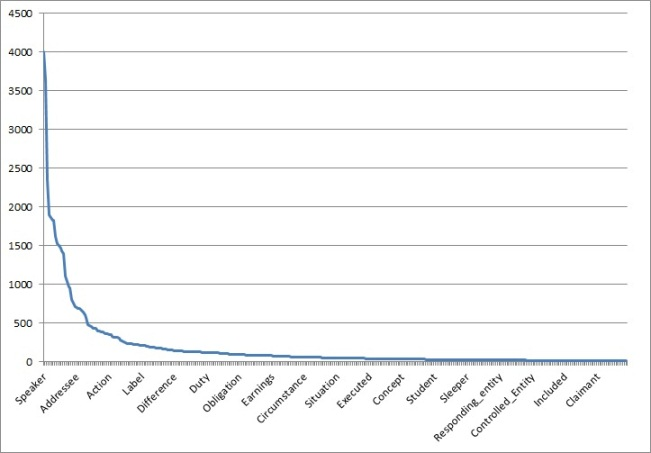
\includegraphics[scale=0.6]{images/roleFrequency.jpg}
		\caption{Verteilung der Rollen im SALSA Korpus 2.0.}
		\label{roleFrequency}
	\end{figure}


\subsection{Kenngrößen der Evaluation}

Der implementierte SRL-Klassifikator wurde hinsichtlich dreier Kenngrößen evaluiert. Abbildung \ref{evalKenngroeszen} zeigt einen annotierten Beispielsatz aus dem SALSA Korpus, an dem die drei unterschiedlichen Fälle markiert wurden.

Die erste Kenngröße erfasst Konstituenten, denen die korrekte Rolle zugewiesen wurde. In Abbildung \ref{evalKenngroeszen} ist der Fall der \textit{exakten Übereinstimmung} in Dunkelgrün dargestellt. 
In einer zweiten Kenngröße wurde jene Konstituenten erfasst, die sowohl im Original als auch in der Annotation eine Rolle zugewiesen wurde, diese jedoch nicht identisch ist. Der Fall \textit{Unabhängig von der Rolle} ist in Abbildung \ref{evalKenngroeszen} Orange markiert. Hier wurde der Konstituente die Rolle Speaker statt der Rolle Message zugewiesen.
Die dritte Kenngröße erfasst das Vorkommen der Originalrollen des Satzes unabhängig davon, welcher Konstituente die Rolle zugewiesen wurde. Wäre ausschließlich der in Abbildung \ref{evalKenngroeszen} blau markierten Konstituente die Rolle Speaker zugewiesen, wäre die Rolle positiv erfasst worden. Dieser Fall wird im Folgenden auch als \textit{Unabhängig von der Position} bezeichnet.

		\begin{figure}[tb!]
			\centering
			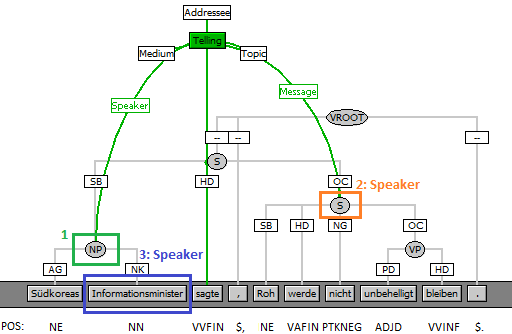
\includegraphics{images/evaluation_kenngroeszen.png}
			\caption{Semantisch-annotierter Beispielsatz mit Beispielen für die drei evaluierten Kenngrößen.}
			\label{evalKenngroeszen}
		\end{figure}


\subsection{Ergebnisse der Evaluation}

Die Ergebnisse der 5-fach Kreuzvalidierung sind in Abbildung \ref{evalKreuzvalidierung} dargestellt. Aufgeteilt nach den drei beschriebenen Kenngrößen, wurde die Precision sowie der Recall gemessen und anschließend der F-Measure berechnet. Bei der \textit{exakten Übereinstimmung} konnte ein F-Measure von 0.62 (Precision: 0.51 Recall: 0.81) erreicht werden. Der F-Measure der zweiten Kenngröße \textit{Unabhängig von der Rolle} fiel mit 0.74 noch höher aus. Dies bedeutet, dass einige Konstituenten korrekt als Inhaber einer Rolle identifiziert wurden, aber ihnen die falsche Rolle zugewiesen wurde. Da der F-Measure mit 0.68 die dritte Kenngröße \textit{Unabhängig von der Position} im Vergleich zur ersten Kenngröße ebenfalls größer ist, wurden stellenweise korrekte Rollen innerhalb eines Satzes annotiert, jedoch an die falschen Konstituenten. 

%TODO: Im Anschluss der Evaluation wurde ausgewertet, wie sehr die getroffenen Annahmen und Einschränkungen das Ergebnis beeinflusst haben. Dabei fiel auf, dass durch die Einschränkung\ldots

		\begin{figure}[tb!]
			\centering
			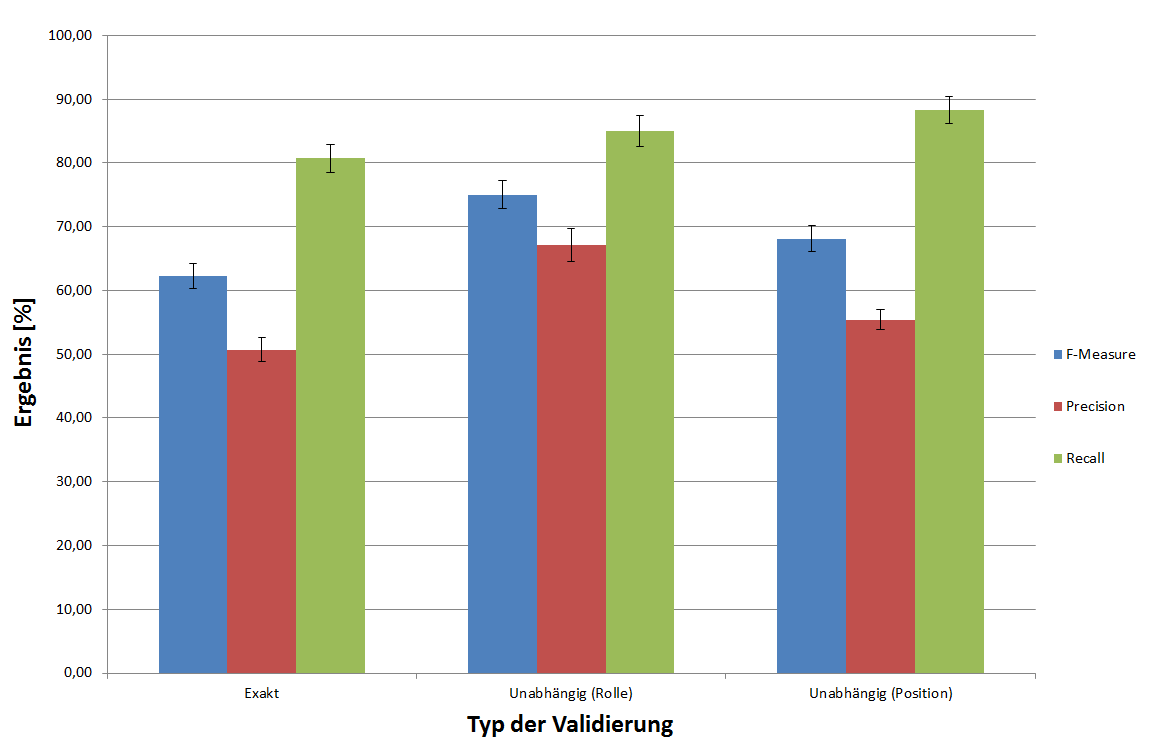
\includegraphics[scale=0.5]{images/ergebnisseKreuzvalidierung.png}
			\caption{Ergebnis der 5-fach Kreuzvalidierung des SRL-Klassifikators bezogen auf die drei Kenngrößen. Dargestellt ist zudem die Standabweichung innerhalb der Kreuzvaliederung.}
			\label{evalKreuzvalidierung}
		\end{figure}

\subsection{Einordnung der Ergebnisse}
		
Der hier entwickelte Ansatz und implementierte SRL-Klassifikator ist das erste und bisher einzige Projekt auf dem SALSA 2.0 Korpus. Dementsprechend gibt es aktuell keine Vergleichsergebnisse anderer Projekte bezüglich der aktuellen Korpusversion.

Ein von \cite{erk2006shalmaneser} entwickeltes Projekt namens SHALMANESER wurde zur automatischen Annotation von Frames und Rollen auf dem SALSA Korpus in der Version 1.0 entwickelt. Der eigentliche Annotationsvorgang ist zweigeteilt. Zuerst findet eine Disambiguierung von Frames statt, bevor die einzelnen Konstituenten bezüglich der gegebenen Frame-Elemente klassifiziert werden. Der während der Klassifikation erreichte F-Measure von 0.600 (Precision: 0.761; Recall: 0.496) ist vergleichbar mit hier erzielten. Leider ist das Vorgehen und die Evaluation unklar.

Ebenso wie SHALMANESER stützten sich auch die Projekte des \textit{CoNLL-2009} Wettbewerbs, welche in \cite{hajivc2009conll} vorgestellt wurden, auf den SALSA Korpus in der Version 1.0. Zusätzlich zum Konstituentenbaum des SALSA Korpus wurde ein Dependendenzgraph mit annotierter Kopf-Konstituente den Projekten zur Verfügung gestellt. Die erreichten Ergebnisse (F-Measure) des Wettbewerbs sind in Tabelle \ref{conll2009} aufgeteilt nach Team und Sprache des jeweiligen Korpus dargestellt. Die für mehrere Sprachen entwickelten Klassifikatoren erreichten auf dem deutschen Korpus einen maximalen F-Measure von 79.71\%. Das schlechteste System erreichte mit einem F-Measure von 59.51\% einen vergleichbaren Wert, wie der hier erstellte SRL-Klassifikator.

	\begin{table}[tb!]
		\centering
		\resizebox{\textwidth}{!}{
			\begin{tabular}{cc|cccccccc}
			\toprule
			\textbf{Rank}   &    \textbf{System}   &    \textbf{Average}   &    \textbf{Catalan}   &    \textbf{Chinese}   &    \textbf{Czech}   &    \textbf{English}   &    \textbf{German} & \textbf{Japanese}   &    \textbf{Spanish} \\
			\midrule
			 1 &    Zhao   &    80.47   &    \textbf{80.32}   &    77.72   &    85.19   &    85.44   &    75.99   &    \textbf{78.15}   &    \textbf{80.46} \\
			 2 &    Nugues   &    80.31   &    80.01   &    \textbf{78.60}   &    \textbf{85.41}   &    \textbf{85.63}   &    \textbf{79.71}   &    76.3   &    76.52 \\
			 3 &    Meza-Ruiz   &    77.46   &    78   &    77.73   &    75.75   &    83.34   &    73.52   &    76   &    77.91 \\
			 4 &    Baoli Li   &    69.26   &    74.06   &    70.37   &    57.46   &    69.63   &    67.76   &    72.03   &    73.54 \\
			 5 &    Moreau   &    66.49   &    65.6   &    67.37   &    71.74   &    72.14   &    66.5   &    57.75   &    64.33\\
			 6 &    Täckström   &    61.27   &    57.11   &    63.41   &    71.05   &    67.64   &    53.42   &    54.74   &    61.51\\
			 7 &    Lin   &    57.18   &    61.7   &    70.33   &    60.43   &    65.66   &    59.51   &    23.78   &    58.87\\
			\bottomrule
			\end{tabular}
		}
		\caption{Ergebniss der CoNLL-2009 Shared Task, SRL-only Task. Die Angaben beziehen sich auf den erreichten F-Measure in Prozent. Fett hervorgehoben ist der jeweils beste Wert pro Sprache. \citep{hajivc2009conll}}
		\label{conll2009}
	\end{table}

\subsection{Einfluss der genutzten Features}

Zusätzlich zu den bereits gewonnenen Erkenntnissen blieb die Frage zu klären, welchen Einfluss die jeweiligen Features besitzen und welches das bedeutendste Feature ist. Zur Bestimmung des Einflusses wurde der Mittelwert der 5-fach Kreuzvalidierung mit allen Features als Basiswert herangezogen. Anschließend wurde jeweils ein Feature samt der komplexen Feature, die dieses enthalten, deaktiviert und die 5-fach Kreuzvalidierung erneut durchgeführt. Abbildung \ref{featureImpact} verdeutlicht den Einfluss der verschiedenen Features. Die Werte geben die Abnahme der Prozentpunkte von F-Measure/Precision/Recall im Vergleich zum festgelegten Basiswert an.
Der \textit{Pfad} mit 21\% im F-Measure sowie das \textit{Nachbar-Kopf-Lemma} mit 19\% im F-Measure sind in der aktuellen Implementierung die bedeutendsten Features. Bezogen auf die Abnahme in Prozentpunkten im Vergleich zum Basiswert hat die syntaktische Kategorie mit 5\% im F-Measure den wenigsten Einfluss. Der Einfluss der beiden bedeutendsten Features beträgt im Vergleich zu den übrigen Features nahezu das Doppelte.

	\begin{figure}[tb!]
		\centering		
		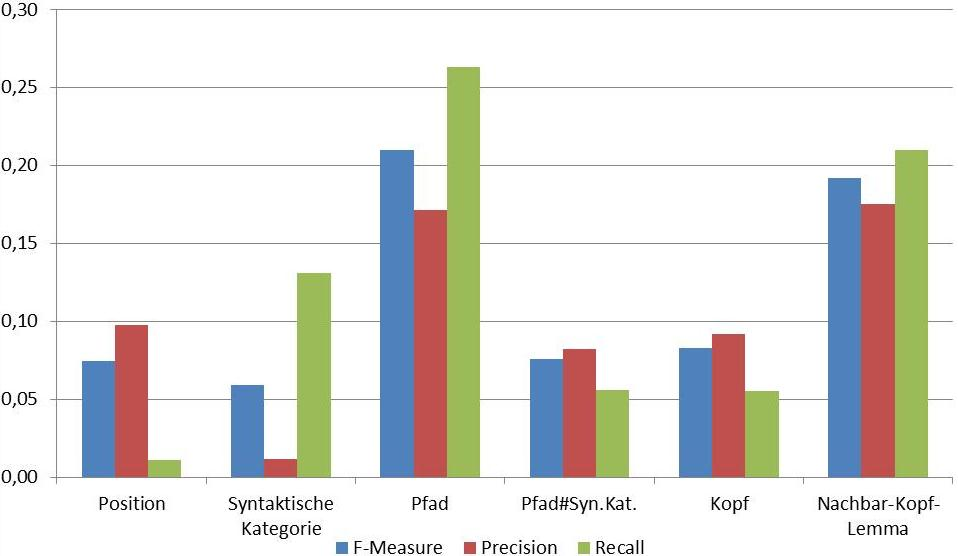
\includegraphics[scale=0.9]{images/featureImpact_sorted.jpg}
		\caption{Der Einfluss der syntaktischen (Position, Syntaktische Kategorie, Pfad \& das aus dem Pfad und der syntaktischen Kategorie zusammengesetzte Feature) und lexikalischen Features (Kopf-Lemma \& Nachbar-Kopf-Lemma). Dargestellt ist die Abnahme in Prozentpunkten im Vergleich zum Basiswert mit allen Features, wenn das jeweilige Feature deaktiviert wurde.}
		\label{featureImpact}
	\end{figure}

\FloatBarrier
\newpage
\section{Zusammenfassung}

Zusammenfassend ist festzuhalten, dass eine automatische Rollenbestimmung
aufgrund von wenigen, rein syntaktischen und lexikalischen Features möglich ist.
Die von \cite{gildea} beschriebenen Features in Verbindung mit einem Naïve-Bayes-Klassifikator konnten erfolgreich adaptiert werden. Einzig die Adaption des Kopf-Features war aufgrund der fehlenden Annotation im genutzten Korpus und der vielen Sonderfälle im entwickelten Regelwerk nicht problemlos möglich.

Die in der Evaluation erreichten Ergebnisse sind vergleichbar mit den Resultaten
einer ähnlichen Arbeit auf einer früheren Version des SALSA Korpus. Zu den in
\cite{hajivc2009conll} vorgestellten und verglichenen Projekten besteht ein
größerer Abstand.


\subsection{Mögliche Erweiterungen und Verbesserungen}

Die bisherige Implementation zur automatischen Annotation von Rollen birgt viel Erweiterungs- und Verbesserungspotential, welches aufgrund der zur Verfügung stehenden Zeit nicht umgesetzt werden konnte.
Eine Verbesserung der aktuellen Implementation wäre eine Änderung des starren Regelwerks zur Bestimmung der Kopf-Konstituenten im Hinblick auf die vielen Sonderfälle, die manuell dem Regelwerk hinzugefügt wurden. Hierbei könnte eine tiefergehende Analyse der Sonderfälle mögliche Abstraktionen von syntaktischen Kategorien aufzeigen, welches eine Minimierung des Regelwerks zur Folge hätte. Das Resultat wäre ein allgemeines, besser nutzbares Regelwerk, welches weiterhin eine hohe Genauigkeit bieten würde.
Eine weitere mögliche Verbesserung wäre die Nutzung eines Dependenzgraphens, welcher in einem zusätzlichen Vorverarbeitungsschritt erzeugt werden müsste. Der Dependenzgraph würde beispielsweise andere Pfade erzeugen, die eindeutiger für bestimmte Rollen sein könnten. 
Bezogen auf die bereits gegebenen Konstiuentenbäume wäre auch eine Nutzung von Tree-Kerneln möglich, welches eine Verarbeitung von Teilbäumen ermöglicht. Die Bestimmung des Pfads zwischen zwei Konstituenten wäre dann überflüssig oder als zusätzliches Features anzusehen.
Um später auch mit ungesehenen Targets arbeiten zu können, wäre eine semantische Abstraktion eben jener mittels des GermaNets möglich. GermaNet\citep{Hamp97germanet} ist das deutsche Pendant zum englischen WordNet\citep{Miller1990} und bietet zahlreiche lexikalisch-semantische Relationen innerhalb des deutschen Grundwortschatzes. Über die Nutzung des GermanNet könnte auch eine Disambiguierung der Frames ermöglicht werden, welche in der aktuellen Implementation übergangen wurden.
 
\newpage
\bibliography{biblio}
\bibliographystyle{natdin}

\end{document}
